\documentclass{beamer}
\usepackage{amsmath}
\usepackage[utf8]{inputenc}
\usepackage{hyperref}
\usepackage{multicol}
\usepackage{hyperref}

\inputencoding{utf8}

\mode<presentation> {
    \usetheme{Madrid}
}

\usepackage{graphicx}
\usepackage{booktabs}

\title[Matematica]{Lenguaje matematico}
\author{Ernesto Rodriguez}
\institute{
    Universidad del Itsmo \\
    \medskip \textit{erodriguez@unis.edu.gt}
}

\date[\today]{}

\begin{document}


\begin{frame}
\frametitle{Lenguaje Matematico}
La matematica se escribe en un lenguaje que:
\begin{itemize}
    \item{Utiliza formulas para representar objetos matematicso.
    e.j. $x^3\forall \psi$}
    \item{Se utiliza una \emph{jerga matematica} en ocasiones
    especiales: ``si y solo si'', ``por lo tanto'', ``Para todo''}
    \item{Se clasifican los enunciados por su proposito: Definicion,
    Lemma, Teorema, Demostraci\'on, Ejemplo}
\end{itemize}
\end{frame}

\begin{frame}
\frametitle{Lenguaje Matematico}
\begin{itemize}
    \item{Se utiliza ``$\wedge$'' y ``$\vee$'' en ves de
    ``y'' y ``o''}
    \item{Se utiliza ``$\neg$'' para negar un enunciado}
    \item{$\forall x.P$ ($\forall x\in S.P$) significa que ``la condicion $P$ la cumple
    para todos los elementos (que pertenecen a $S$)''}
    \item{$\exists x.P$ ($\exists x\in S.P$) significa que ``existe
    al menos un elemento (que pertenece a $S$) que cumple con la condici\'on
    $P$''}
    \item{$\neg\exists x.P$ ($\neg\exists x\in S.P$) significa ``no
    existe un x (que pertenece a $S$) que cumple la condicion $P$''}
    \item{$\exists^{1} x.P$ ($\exists^{1} x \in S.P$) significa ``existe exactamente
    un objeto (en S) que cumple la condicion $P$''}
    \item{``ssi'' es abreviaci\'on para ``si y solo si''}
    \item{El simbolo $\Rightarrow$ significa ``implica''}
\end{itemize}
\end{frame}

\begin{frame}
\frametitle{Ejemplos}

\begin{itemize}
    \item{$\forall x\exists y.x=y \Leftrightarrow \neg(x\neq y)$ significa
    ``Para todo $x$, existe un $y$, tal que $x=y$, ssi (si y solo
    si) no se cumple que $x\neq y$''}
\end{itemize}

\end{frame}

\begin{frame}
\frametitle{Axiomas de Peano en lenguaje matematico}
Los aximoas de Peano en lenguaje matematico: Si escribimos
``$n\in\mathbb{N}_1$'' para ``$n$ es un numero natural unario'', y
``$P(n)$'' ``$n$ tiene la propiedad $P$'', podemos escribir:
\begin{enumerate}
\item{El cero es un numero natural unario: $o\in \mathbb{N}_1$}
\item{Todo numero tiene un sucesor diferente de el$\forall n \in \mathbb{N}_1.s(n)\in\mathbb{N}_1\wedge n\neq s(n)$}
\item{El cero no es un succesor $\neg(\exists n \in\mathbb{N}_1.o=s(n))$}
\item{Diferentes numeros tienen diferentes sucesores$\forall n \in\mathbb{N}_1.\forall m\in\mathbb{N}_1.n\neq m\Rightarrow(n)\neq s(m)$}
\item{Inducci\'on: $\forall P.(P(p)\wedge(\forall n \in \mathbb{N}_1
.P(n)\Rightarrow P(s(n))))\Rightarrow (\forall m\in\mathbb{N}_1.P(m))$}

\end{enumerate}
\end{frame}

\begin{frame}
\frametitle{Definiciones}
\begin{itemize}
    \item{Se utiliza el simbolo $:=$ para definir un objeto}
    \item{Por ejemplo, podemos definir el simbolo ``$1$'' asi: $1:=s(o)$}
    \item{Asi se define la union de conjuntos: $A\cap B:=\{
        x|x\in A \wedge x\in B\}$}
\end{itemize}
\end{frame}

\begin{frame}
\frametitle{Letras Griegas}
Las letras griegas se utilizan a menudo como variables en
lenguaje matematico:
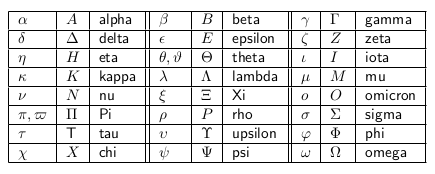
\includegraphics[width=10cm]{greek.png}
\end{frame}

\end{document}